% -*-LaTeX-*-
\documentclass{sig-alternate-10pt}
\clubpenalty=10000
\widowpenalty = 10000

\usepackage{times,latexsym}
\usepackage[caption=false]{subfig}
\usepackage[sort]{cite}
\usepackage[hyphens]{url}
\usepackage{lastpage}
\usepackage{array, verbatim}
\usepackage{mdwlist}
\hyphenpenalty=5000
\tolerance=1000

\usepackage{multirow}

\newcommand\todo[1]{}

\setlength{\pdfpagewidth}{8.5in}
\setlength{\pdfpageheight}{11in}

\usepackage{ifpdf}
\usepackage{graphicx}
\graphicspath{{./figs2011/}}

\ifpdf
  \DeclareGraphicsExtensions{.pdf}
\else
  \DeclareGraphicsExtensions{.eps}
\fi

\usepackage{mathtools}
\usepackage{alltt}
\usepackage{wasysym}
\usepackage{listings}
\usepackage{array}
%\usepackage{pdfcomment}
%\usepackage[rgb]{xcolor}

\renewcommand\floatpagefraction{.9}
\renewcommand\topfraction{.9}
\renewcommand\bottomfraction{.9}
\renewcommand\textfraction{.1}   
\setcounter{totalnumber}{50}
\setcounter{topnumber}{50}
\setcounter{bottomnumber}{50}

\newcommand{\enote}[2]{({\bf{#1:} \it{#2}})}
%\newcommand{\enote}[2]{}


\begin{document}

\title{Broadband Access in the US}
\author{
Zachary Bischof\\
Christopher Moran
}
  
\maketitle

%******************************************************************************
\begin{abstract}
 
Understanding the quality of Internet services that are avaible to customers is
import to government organizations surveying broadband availability in their 
country.

In this work, we study the quality (in terms of download throughput) of
broadband services available across the US. We used data provided by the FCC to
analyze trends in the quality of services available to customers in a region.
We compare this against consesus data, looking at how the quality of broadband
services relates to the median average income, finding that, in general,
regions with a higher median income have wider access to faster services.
However, using data collected by Ono, a BitTorrent extension, we find that
these services are not widely used, or evident, in BitTorrent traffic.

\end{abstract}


%******************************************************************************
\section{Problem Statement}
\label{sec:statement} 



%******************************************************************************
\section{Prior Work}
\label{sec:prior-work}


 
%******************************************************************************
\section{Approach}
\label{sec:approach} 



%******************************************************************************
\section{Results}
\label{sec:results} 

\begin{figure}
\centering
        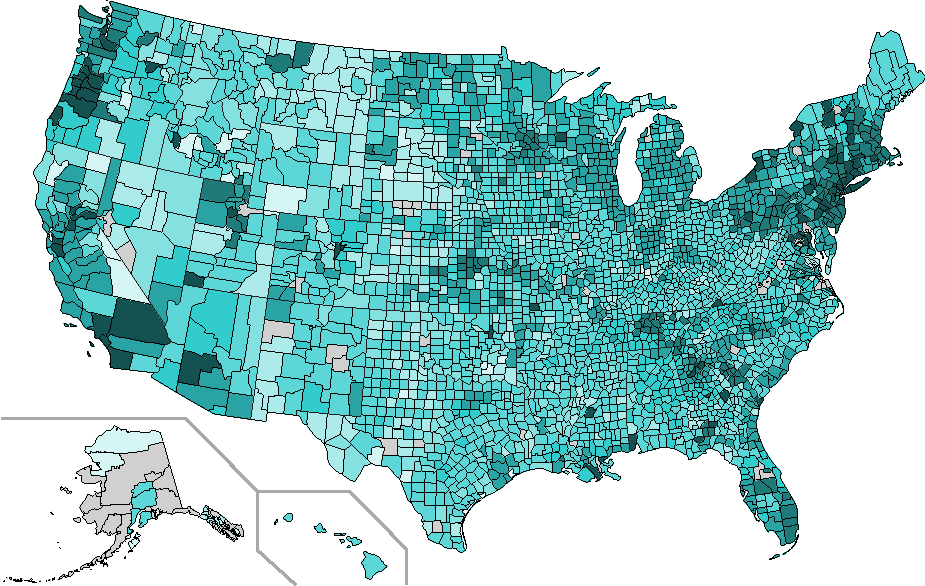
\includegraphics[width=0.9\linewidth]{figs/counties_maxDown.pdf}
  \caption{}
  \label{fig:services-hist}
\end{figure}

\begin{figure}
\centering
        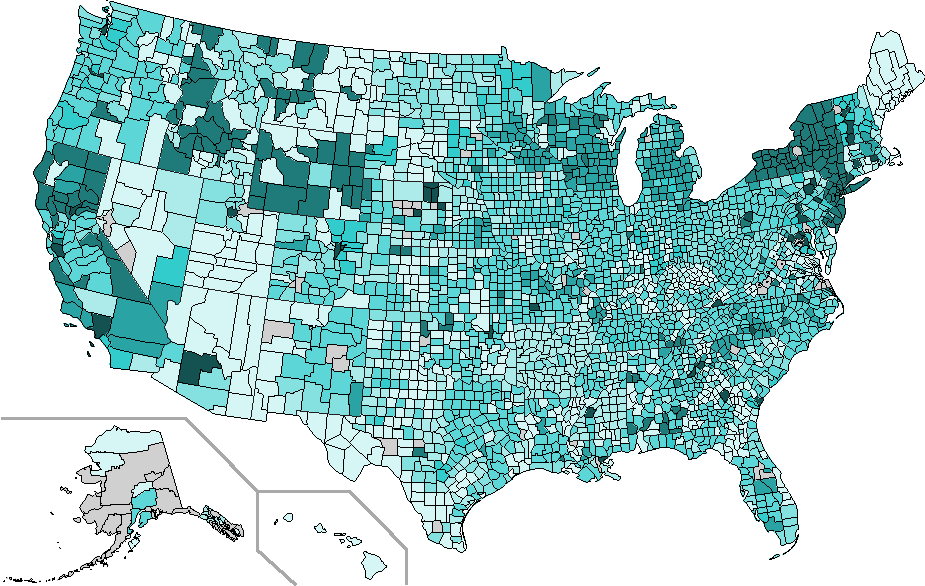
\includegraphics[width=0.9\linewidth]{figs/counties_typDown.pdf}
  \caption{}
  \label{fig:services-hist}
\end{figure}


\begin{figure}
\centering
        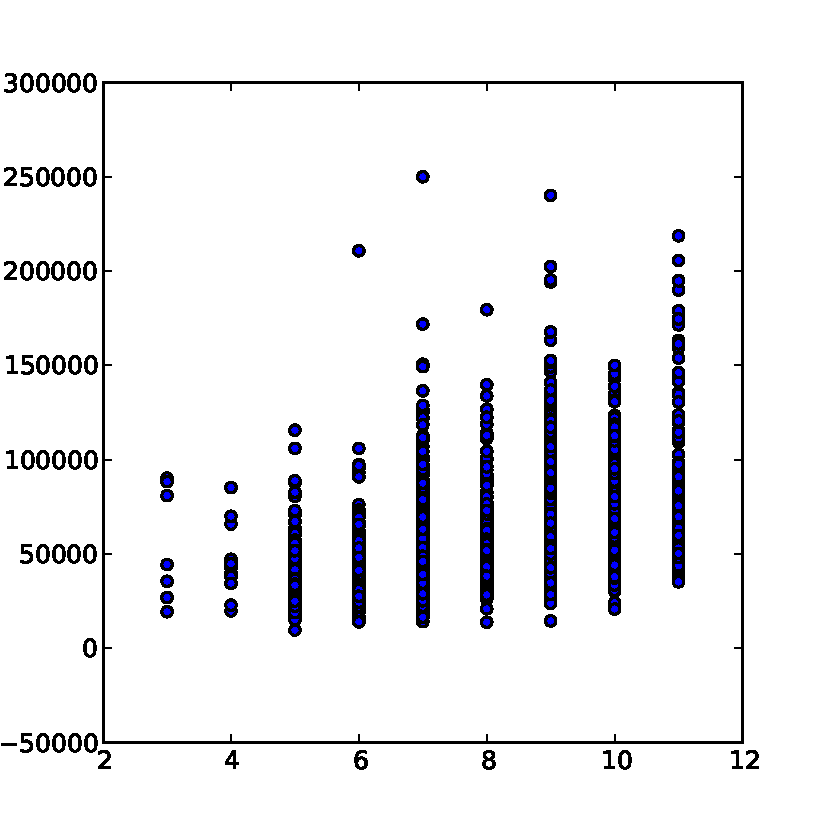
\includegraphics[width=0.9\linewidth]{figs/maxIncome_maxDown.pdf}
  \caption{}
  \label{fig:services-hist}
\end{figure}

\begin{figure}
\centering
        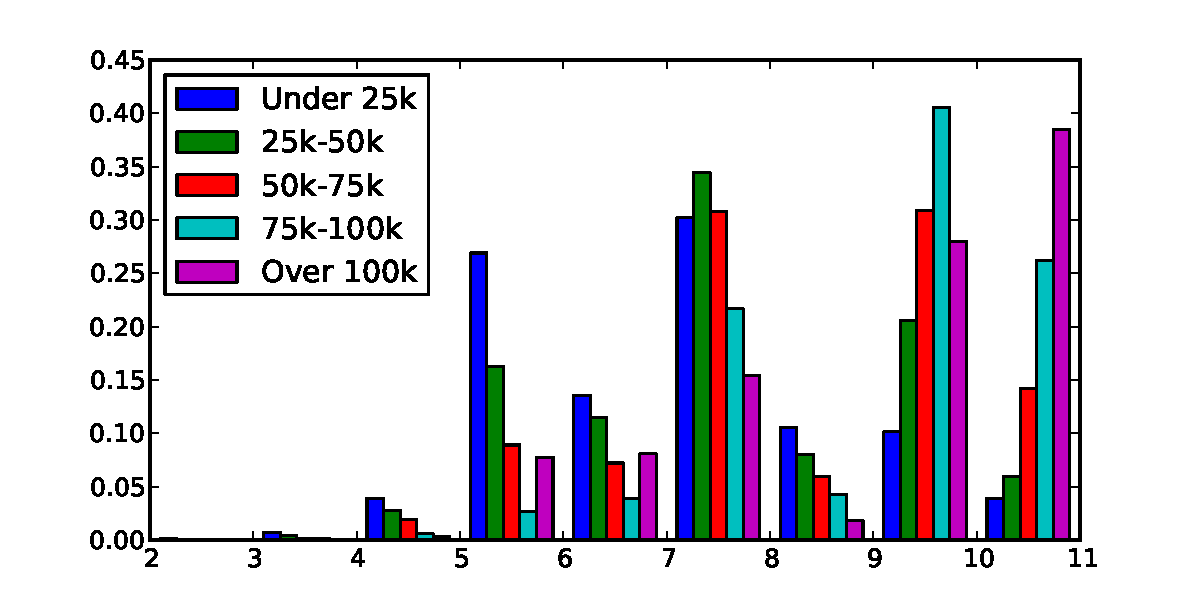
\includegraphics[width=0.9\linewidth]{figs/all_hist.pdf}
  \caption{}
  \label{fig:services-hist}
\end{figure}

\begin{figure}
\centering
        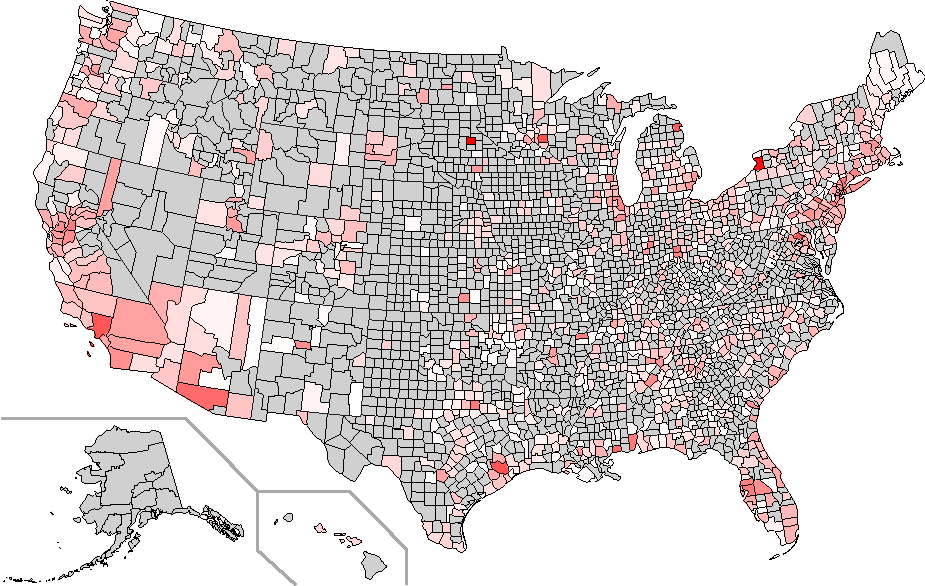
\includegraphics[width=0.9\linewidth]{figs/counties_btMaxDown.pdf}
  \caption{}
  \label{fig:services-hist}
\end{figure}

\begin{figure}
\centering
        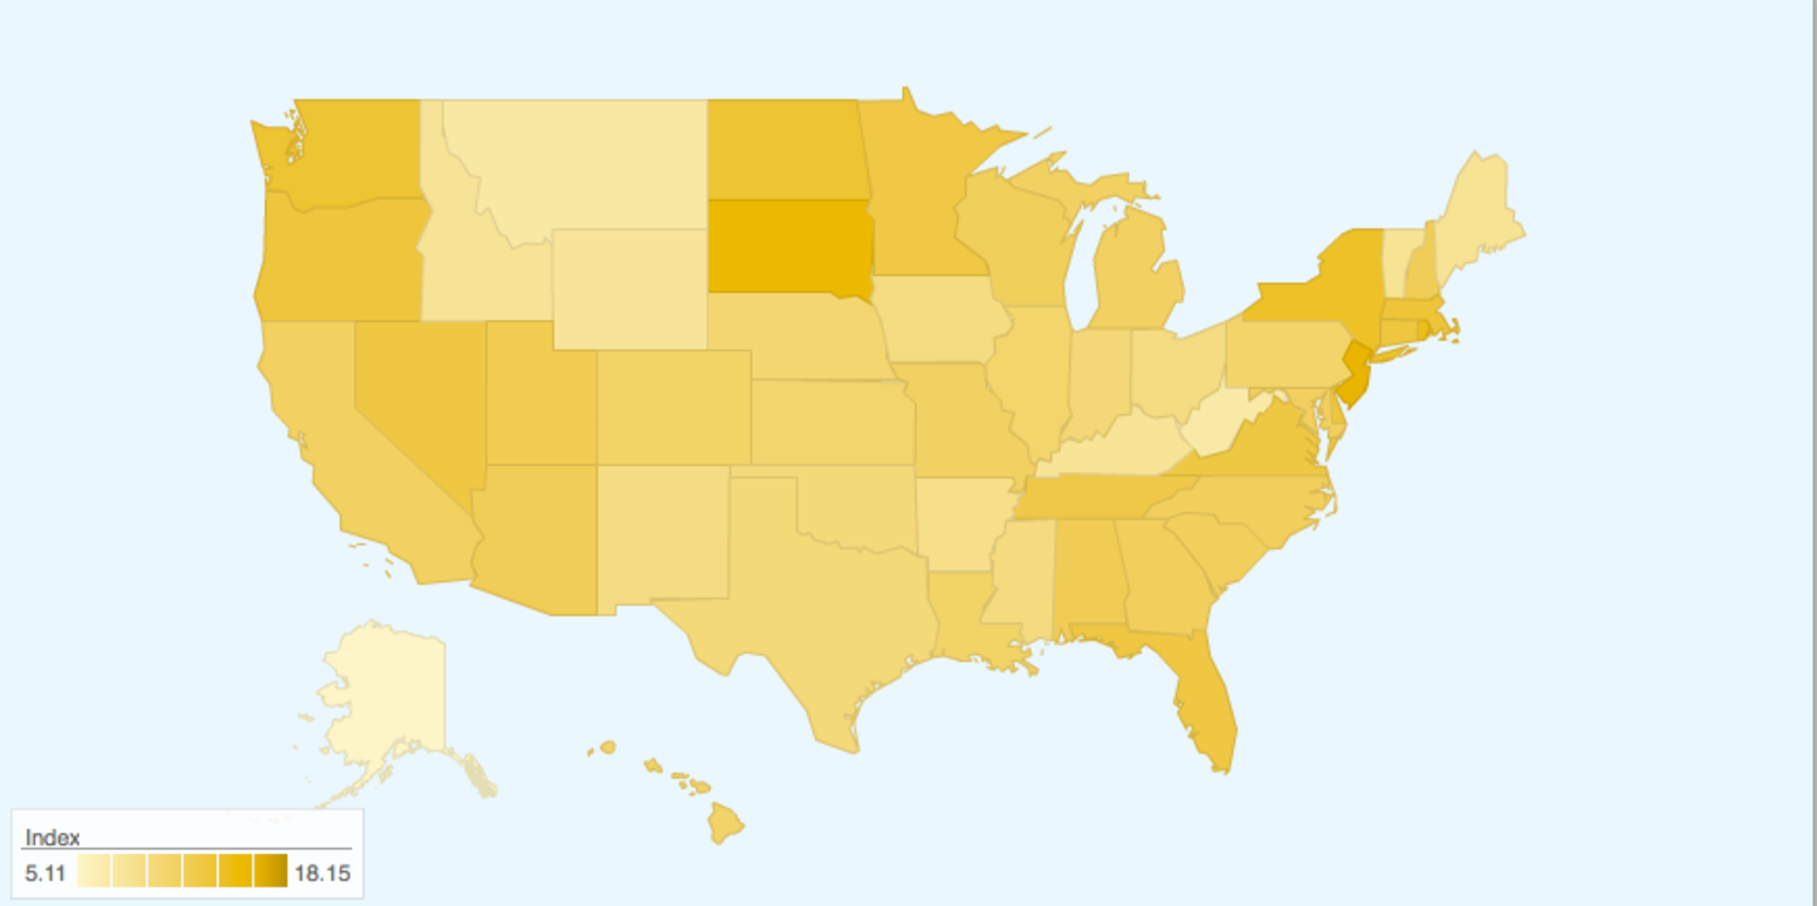
\includegraphics[width=0.9\linewidth]{figs/map.pdf}
  \caption{}
  \label{fig:services-hist}
\end{figure}

%******************************************************************************
\section{Future Work}
\label{sec:future-work} 



%******************************************************************************
\section{Conclusion}
\label{sec:conclusion} 



\end{document}
